\section{結果を描画する:net2g} \label{sec:quicklook}
%####################################################################################

ここでは、
プロセス毎に分割された{\netcdf}形式の出力ファイル(\verb|history.**.nc|
\footnote{gpviewがインストールされている場合、gpviewを使って作図することも出来る
gpviewならばhistoryデータを変換することなく直接作図することができるため、クイックチェックに適している。}
)を
{\grads}で読み込めるように1つのバイナリファイルにまとめる
\verb|netcdf2grads (略して、net2g)|の使い方と、変換した{\grads}バイナリデータを使って
結果の確認を行う。


\subsubsection{{\grads}バイナリに変換}
%-----------------------------------------------------------------------------------
プロセスごとに分割された{\netcdf}形式のhistoryファイルから
{\grads}バイナリ変換するには、\verb|net2g|を使用する。
詳細な使用方法は \ref{sec:net2g}節を参照頂くこととし、
ここでは最低限の手続きのみ説明する。\\

まず、\verb|net2g|ディレクトリへ移動する。
\begin{verbatim}
 $ cd ${Tutorial_DIR}/real/experiment/net2g
 $ ls
    net2g -> ../../../../../util/netcdf2grads_h/net2g
    net2g.2D.d01.conf
    net2g.3D.d01.conf
\end{verbatim}
中には設定ファイルとバイナリファイルがあり、
バイナリファイルは\ref{sec:source_net2g}節のコンパイルにより作成された
実行ファイルにリンクが貼られている。\\

ここでは例として、2次元変数のMSLP、PRECの変換と、
3次元変数のU、Vを850hPa、500hPa、200hPa面で抽出して変換する手順について説明する。
2次元変数のための設定ファイルは \verb|net2g.2D.d01.conf| に、
3次元変数のための設定ファイルは \verb|net2g.3D.d01.conf| に用意している。

\verb|netcdf2grads_h|実行時のプロセス数は、
計算実行時に使用したプロセス数の約数である必要がある。
ここでは、計算に用いた時と同じ4プロセスを使用する。
net2gでは2次元変数と3次元変数を同時に変換することはできないため、
別々に実行する。
\begin{verbatim}
 $ mpirun -n 4 ./net2g net2g.2D.d01.conf
 $ mpirun -n 4 ./net2g net2g.3D.d01.conf
\end{verbatim}
エラーメッセージがなく、下記のメッセージだけが標準出力へ表示されていれば正常に変換完了である。\\

\noindent {\gt
\fbox{
\begin{tabularx}{150mm}{l}
\verb|+++ MPI COMM: Corrective Finalize| \\
\end{tabularx}
}}\\

成功すれば、下記のファイルが作成される。
\verb|**.ctl|は {\scalerm} のXY格子座標のctlファイル、
\verb|**lccr.ctl|は緯度経度座標で作図するためのctlファイルである。

\begin{verbatim}
  MSLP_d01z-2d.ctl
  MSLP_d01z-2d.grd
  MSLP_d01z-2d_lccr.ctl
  PREC_d01z-2d.ctl
  PREC_d01z-2d.grd
  PREC_d01z-2d_lccr.ctl
  PRES_d01z-3d.ctl
  PRES_d01z-3d.grd
  PRES_d01z-3d_lccr.ctl
  U_d01z-3d.ctl
  U_d01z-3d.grd
  U_d01z-3d_lccr.ctl
  V_d01z-3d.ctl
  V_d01z-3d.grd
  V_d01z-3d_lccr.ctl
\end{verbatim}




\subsubsection{計算結果の確認}
%-----------------------------------------------------------------------------------

%\verb|${Tutorial_DIR}/real/data|ディレクトリに用意してあるので、
%サンプルとして利用してほしい。\footnote{今後、緯度経度座標で描画するためのctlファイルを出力できるようにする予定。}
%\begin{verbatim}
% $ cp ../../data/*_lcc.ctl ./
% $ ls
%    MSLP_d01z-2d_lcc.ctl
%    PREC_d01z-2d_lcc.ctl
%    U_d01z-3d_lcc.ctl
%    V_d01z-3d_lcc.ctl
%\end{verbatim}

計算結果確認用の図を作成するための\grads スクリプト\verb|checkfig_real.gs|を使って作図する。
\begin{verbatim}
 $ cp ../../data/checkfig_real.gs ./
 $ grads -blc checkfig_real.gs
\end{verbatim}
成功すると、下記の図が作成される。
なお、\grads のバージョンによって文法が異なるので、Warningが出る場合は、適宜変更する。
\begin{verbatim}
  real_mslp.png
  real_prec.png
  real_wind.png
\end{verbatim}
計算と変換が成功していれば、下記と同じ図が描画される。

\proofcomment{(足立)最後のチェックで図の入れ替え!!!}

\begin{figure}[h]
\begin{center}
  \includegraphics[width=0.55\hsize]{./figure/real_mslp.eps}\\
  \caption{計算開始から6時間後の海面更正気圧}
  \label{fig:real_mslp}
\end{center}
\begin{center}
  \includegraphics[width=0.55\hsize]{./figure/real_prec.eps}\\
  \caption{計算開始から6時間後の降水フラックス}
  \label{fig:real_prec}
\end{center}
\begin{center}
  \includegraphics[width=0.55\hsize]{./figure/real_wind.eps}\\
  \caption{計算開始から6時間後の500hPaの風速と風ベクトル}
  \label{fig:real_wind}
\end{center}
\end{figure}

